\documentclass[10pt]{article} % For LaTeX2e

% ── TMLR camera-ready ────────────────────────────────────────────────────────
% The [accepted] option de-anonymises the paper and prints the TMLR
% certification header + the OpenReview link defined below.
\usepackage[accepted]{tmlr}

\usepackage[utf8]{inputenc}
\usepackage[T1]{fontenc}
\usepackage{hyperref}
\usepackage{url}
\usepackage{booktabs}
\usepackage{amsfonts}
\usepackage{amsmath}
\usepackage{amssymb}
\usepackage{nicefrac}
\usepackage{microtype}
\usepackage{xcolor}
\usepackage{graphicx}
\usepackage{multirow}
\usepackage{algorithm}
\usepackage{algpseudocode}

% Macros
\newcommand{\dmodel}{d_{\text{model}}}
\newcommand{\dinner}{d_{\text{inner}}}
\newcommand{\dstate}{d_{\text{state}}}
\newcommand{\dattn}{d_{\text{attn}}}
\newcommand{\nhormones}{n_{\text{h}}}
\newcommand{\TODO}[1]{\textcolor{red}{[TODO: #1]}}
\newcommand{\TBD}[1]{\textcolor{red}{[#1]}}

\title{When Routing Doesn't Move the Loss: Genre-Associated Routing Specialisation in a 125M-Parameter Hybrid Language Model}

% ── Authors (de-anonymised) ──────────────────────────────────────────────────
% CONFIRM before submitting: (1) the email you want publicly listed, and
% (2) your affiliation. "Independent Researcher" is a placeholder default —
% edit it if you have an institutional affiliation.
\author{\name Ariet Jha \email ariet.jha@gmail.com \\
      \addr Independent Researcher}

% ── Camera-ready metadata (CONFIRM the publication month) ────────────────────
\def\month{10}   % 2-digit publication month
\def\year{2026}  % 4-digit publication year
\def\openreview{\url{https://openreview.net/forum?id=uZuaQlxfwG}}

\begin{document}

\maketitle

\begin{abstract}
We construct a controlled setting in which an architectural channel in a hybrid state-space/attention language model is free to organise its internal representations without measurably affecting the optimisation objective. The channel is \emph{hormone routing}: a token-conditional softmax-gated linear combination of a small bank of frozen direction vectors, added to the residual stream after each attention block. We pretrain a 125M-parameter Mamba/MQA hybrid on FineWeb-Edu under a fixed 2B-token budget across five variants of this channel --- extracted directions, random unit vectors, vectors extracted from a randomly-initialised model, and a frozen gate at $1.0$. The router develops semantically-coherent per-genre routing specialisation in every variant, with maximum pairwise $L_1$ distance between genre routing distributions in $0.6$--$1.6$ (a permutation-null baseline places the chance level below $0.1$; see Section~\ref{sec:analysis}). The variant of \emph{highest} specialisation strength is the one whose gate the model cannot modulate. \textbf{Specialisation strength does not predict downstream loss}: the four properly-initialised variants converge to identical validation perplexity ($26.13$). To probe whether this loss-invariance is a ceiling or a regime the model actively absorbs, a sixth variant adds a forced non-zero gate initialisation and a non-trainable $3\times$ amplification. The model drifts the gates downward and shrinks the per-hormone magnitudes, but the residual perturbation it cannot suppress --- $\approx 2\times$ the unforced regime --- does not damage loss either. We refer to the regime in which the gated injection is consistently absorbed without affecting predictions as a \emph{homeostatic envelope}. The envelope is wider than the unforced variants naturally select; the loss-relevant axis is the training schedule (introducing routing during base pretraining rather than as a continuation raises validation perplexity by $+2.07$ PPL). An isolation ablation reported in Section~\ref{subsec:noext-cont} decomposes this damage as $\approx 79\%$ schedule ($+1.64$ PPL) and $\approx 21\%$ bank content ($+0.43$ PPL): schedule is the dominant factor by roughly $4\!:\!1$, but an uninformative bank contributes a small measurable residual even in the staged regime. All results are at a single scale ($125$M parameters, $2$B tokens, one architecture family, single seed per variant); we hedge accordingly. Appendix~\ref{app:ia} sketches a second architectural mechanism --- intracellular attention, slot attention inside the SSM scan --- as future work.
\end{abstract}

\section{Introduction}
\label{sec:intro}

Architectural mechanisms in language models are typically introduced with a presumed contribution to the optimisation objective: a new attention variant, normalisation, or gating scheme is judged by whether it lowers the loss. We instead investigate a setting in which an architectural channel is free to develop structured internal representations \emph{without} measurably affecting the loss, and ask what such a channel does.

Our setting is built on hybrid state-space/attention language models~\citep{gu2023mamba,vaswani2017attention,lieber2024jamba,glorioso2024zamba,park2024empirical}. Inside this backbone we introduce \emph{hormone routing}, a parameter-efficient channel that injects a token-conditional gated combination of a small bank of frozen direction vectors into the residual stream after each attention block. The bank is non-trainable; the router and gate are. The mechanism adds under $0.01\%$ of base parameters and is gated such that, at initialisation, the modification is an exact no-op and the hybrid backbone is recovered bit-for-bit. Directions are obtained from a partially-trained Stage-1 checkpoint via document-style contrast-pair extraction~\citep{turner2023activation,rimsky2024steering,zou2023representation}.

\paragraph{The empirical phenomenon.} Across every hormone-routing variant we tested at the $125$M-parameter, $2$B-token scale --- with extracted directions, with random unit vectors, with the gate frozen at $1.0$, and with directions extracted from a randomly-initialised model --- the router converges to a strongly genre-discriminative routing distribution (max pairwise $L_1$ distance across six text genres, at the engaged upper attention layer: $0.96$--$1.56$, vs $0.0$ for uniform and well above a permutation-null 99th percentile of $0.62$; see Section~\ref{sec:analysis}). The specialisation is qualitatively interpretable in the variant where directions carry semantic labels (news $\to$ urgency, fiction $\to$ curiosity, code $\to$ skepticism) and structurally analogous in the variants where they do not. Yet none of these variants moves the validation perplexity needle: all properly-initialised variants achieve identical val PPL ($26.13$), and loss trajectories trace the same curve to within $10^{-3}$ across all of Stage 2. Training the same router from scratch with hormones in place from step $0$ damages the loss by $+2.07$ PPL even though it still develops similar specialisation. \textbf{The loss-relevant variable is when the perturbation is introduced, not what it contains.}

\paragraph{Probing the regime.} Two readings are worth distinguishing: either the perturbation magnitude in the unforced variants is too small to matter (capacity-bottlenecked), or the architecture has actively absorbed a non-negligible injection (structural homeostasis). We probe this with a sixth variant with a forced non-zero gate initialisation and a non-trainable $3\times$ amplification, intended to force a larger effective perturbation. In practice the model drifts the gates downward and shrinks per-hormone magnitudes, so even with $\alpha$ fixed the residual perturbation it actually introduces stays under $0.2\%$ of the residual-stream norm --- and validation loss is undamaged at the matched training step. We stress the limitation this exposes: because the model keeps the effective injection so small, this experiment does \emph{not} rule out the capacity-bottlenecked reading. A tiny perturbation being loss-invariant is exactly what that reading predicts. What the forced variant does show is that the invariance survives an explicit attempt to enlarge the injection, and that the model's response is to shrink the channel rather than exploit it. We use \emph{homeostatic envelope} descriptively throughout, for the range of effective injection magnitudes we have probed without detecting a loss difference --- not for an identified absorption mechanism.

\paragraph{Contributions.}
\begin{itemize}
    \item \textbf{Empirical (primary)}: under the tested conditions, no detectable difference in validation loss across routing-channel variants that differ markedly in specialisation, in a 125M-parameter hybrid LM. Five hormone-routing variants on a 2B-token budget all develop strongly genre-discriminative routing, yet specialisation strength does not predict validation perplexity. A sixth, forced-engagement variant shows the loss-invariance persists under an attempt to enlarge the injection; because the model shrinks the channel in response (keeping $\|\Delta h\|/\|h\| < 0.2\%$), we do not claim to rule out a capacity bottleneck. The one axis along which we \emph{do} observe measurable loss damage is training schedule.
    \item \textbf{Architectural (primary)}: \emph{hormone routing}, a token-conditional softmax-gated routing channel, plus a document-style contrast-pair extraction protocol that recovers behavioural directions from the base model itself.
\end{itemize}

Appendix~\ref{app:ia} sketches a second architectural mechanism --- \emph{intracellular attention}, slot attention over the $\dstate$ memory cells inside the SSM scan --- and reports a preliminary engagement signal at a reduced token budget. We treat this as future work rather than a claim of the paper: full-budget evaluation requires a fused CUDA kernel that is out of scope here.

The rest of the paper situates the work (Section~\ref{sec:related}), gives the hybrid backbone (Section~\ref{sec:arch}), presents hormone routing (Section~\ref{sec:hormone}), reports the empirical study (Section~\ref{sec:experiments}), and characterises what the router learns (Section~\ref{sec:analysis}).

\section{Related Work}
\label{sec:related}

\paragraph{State-space models and hybrids.}
Structured state-space models~\citep{gu2021combining,gu2022efficiently,gupta2022diagonal} reformulate sequence mixing as a parameterised linear dynamical system; Mamba~\citep{gu2023mamba} adds input-dependent selectivity to the discretisation step, input matrix, and readout. Pure-SSM models lag pure-attention transformers on tasks requiring precise in-context recall~\citep{jelassi2024repeat,arora2023zoology}; hybrids interleave attention layers among many SSM layers~\citep{lieber2024jamba,glorioso2024zamba}, and~\citet{park2024empirical} show that even a single attention layer per block recovers most of the lost expressivity. We adopt a 5:1 SSM-to-attention ratio with multi-query attention~\citep{shazeer2019fast} and rotary positional embeddings~\citep{su2021roformer}. Our contributions are orthogonal to the choice of mixing ratio.

\paragraph{Activation steering and representation engineering.}
A growing body of work shows that LLM behaviour is modulated by a small number of linear directions in the residual stream. \citet{zou2023representation} introduce representation-engineering as a framework for reading and writing such directions; \citet{turner2023activation} and \citet{rimsky2024steering} demonstrate that adding a difference-of-means vector --- computed from contrastive prompts --- can steer attributes like truthfulness, refusal, and persona at inference time. Earlier work on contrast-consistent search~\citep{burns2022discovering} and probing~\citep{alain2017understanding} establishes that interpretable axes are present in unmodified models. All of this work applies the directions \emph{post-hoc} at inference time. Our hormone-routing module instead re-injects extracted directions \emph{during pretraining} through a learned router; the directions themselves stay frozen.

\paragraph{Routing, mixture-of-experts, and soft prompts.}
MoE models~\citep{shazeer2017outrageously,fedus2022switch,jiang2024mixtral} use learned routers to dispatch tokens to specialised expert subnetworks. Our hormone router is structurally analogous --- a linear-then-softmax map from the hidden state to a distribution over a small fixed set --- but the ``experts'' here are frozen direction vectors of dimension $\dmodel$, not parameter banks. Soft prompts~\citep{lester2021power,li2021prefix} likewise use a small bank of $\dmodel$-dimensional vectors to modulate behaviour, but those vectors are prefix tokens exposed to attention rather than residual-stream additions, and are fixed across the sequence rather than token-conditional.

\paragraph{Routed representation-intervention methods.}
A concurrent line of work trains lightweight routers or intervention networks over frozen representations. Representation Finetuning (ReFT)~\citep{wu2024reft} trains low-rank interventions in the residual stream, with variants such as CS-ReFT~\citep{wu2024csreft} that compose subspace-level interventions. \citet{zhang2024guidinggiants} propose lightweight controllers for weighted activation steering in LLMs. Most directly related to our setup, RISER~\citep{postmus2024riser} trains a lightweight router over activation vectors for instruction-following behaviour. Our contribution shares the training-a-router-over-frozen-directions design pattern with RISER but differs on setting and framing in three ways: (i) we operate in a continued-pretraining hybrid-SSM setting rather than a supervised-finetuning transformer setting; (ii) the direction vectors we route over are extracted via document-style contrast pairs from the base model itself, not defined externally; and (iii) our finding is about the \emph{decoupling} of the router's specialisation from validation loss, not about the router's use as an intervention interface. The observation that routing structure can vary substantially without a detectable change in validation loss is orthogonal to the mechanism-design aims of these methods.

\paragraph{Probing and the structure-vs-task gap.}
A long line of work probes neural network internals for learned structure not obviously demanded by the training objective~\citep{alain2017understanding,hewitt2019designing,belinkov2022probing}. \citet{hewitt2019designing} caution that high-capacity probes can recover arbitrary structure regardless of whether the network exploits it. Our routing-specialisation finding is in the same spirit but at a different locus: the routing module is not a post-hoc probe but a built-in architectural channel, and the structure it develops is a property of the model's own forward pass. The decoupling we observe between specialisation strength and downstream loss is stronger than ``the probe finds structure that does not matter'' --- it is ``the model itself produces and uses structure that does not matter for its training objective,'' at least at the scale we examine.

\section{Architecture}
\label{sec:arch}

We use a hybrid Mamba/MQA backbone of $L$ residual layers with a fixed 5:1 SSM-to-attention pattern (five SSM layers between every attention layer). All layers share hidden width $\dmodel$, use RMSNorm~\citep{zhang2019root}, and tie word embeddings with the LM head.

\paragraph{SSM layers.} Each SSM layer applies pre-norm and a Mamba-1 selective block~\citep{gu2023mamba}, with no separate channel-mixing MLP. The block projects to twice the inner width ($\dinner = 2\dmodel$), applies a causal depthwise convolution, and runs a selective scan parameterised by an input-dependent step $\Delta_t$, input matrix $B_t \in \mathbb{R}^{\dstate}$, readout $C_t \in \mathbb{R}^{\dstate}$, and per-channel diagonal $A \in \mathbb{R}^{\dinner \times \dstate}$ in log-space. The recurrent state $h_t \in \mathbb{R}^{\dinner \times \dstate}$ updates as $h_t = \Delta_t A \odot h_{t-1} + \Delta_t B_t \odot x_t$ with readout $y_t = h_t C_t^\top + D \odot x_t$. Appendix~\ref{app:ia} sketches an alternative in which the linear contraction $h_t C_t^\top$ is replaced with attention over the $\dstate$ slots (future work).

\paragraph{Attention layers.} Pre-norm followed by multi-query attention~\citep{shazeer2019fast} with a single shared key/value head, RoPE~\citep{su2021roformer} on Q/K, and a SwiGLU~\citep{shazeer2020glu} MLP of inner width $d_{\text{ff}} = \lceil \nicefrac{8}{3}\dmodel \rceil$ rounded to a multiple of $64$. Section~\ref{sec:hormone}'s hormone routing adds a third residual after the MLP: $x \leftarrow x + \text{Hormone}(x)$.

\paragraph{Configurations.} All experiments use the \textsc{tiny} configuration ($\dmodel = 1024$, $L = 12$, $\dinner = 2048$, $\dstate = 16$, eight query heads, one shared KV head, head dim $128$, $\approx 125$M parameters). \textsc{small} ($350$M) and \textsc{medium} ($770$M) variants are defined for future scaling experiments (Table~\ref{tab:configs}).

\begin{table}[h]
\centering
\caption{Backbone configurations. All sizes share $\dstate = 16$, $\dattn = 16$, head dim $128$, MQA, 5:1 SSM:Attn pattern.}
\label{tab:configs}
\small
\begin{tabular}{lccccc}
\toprule
Name & Params & $\dmodel$ & $L$ & $n_{\text{heads}}$ & SSM/Attn \\
\midrule
\textsc{tiny}   & $\sim$125M & 1024 & 12 & 8  & 10/2 \\
\textsc{small}  & $\sim$350M & 1536 & 18 & 12 & 15/3 \\
\textsc{medium} & $\sim$770M & 2048 & 24 & 16 & 20/4 \\
\bottomrule
\end{tabular}
\end{table}

\section{Intracellular Attention (future work)}
\label{sec:intracellular}

We additionally sketch a second architectural mechanism, \emph{intracellular attention} (IA): slot attention over the $\dstate$ memory cells inside the SSM scan, with the same zero-init gating discipline as hormone routing. IA is treated in this paper as future work rather than a validated contribution --- full-budget training is not tractable within our compute budget without a fused CUDA kernel, and the empirical evidence we have is insufficient to support conclusions about IA's effect on the loss at scale. The architecture, algorithmic pseudocode, cost analysis, and a preliminary $12$M-token engagement signal are reported in Appendix~\ref{app:ia}. The rest of the paper reports experiments on hormone routing only.

\section{Hormone Routing}
\label{sec:hormone}

\subsection{The hormone routing module}

Let $V \in \mathbb{R}^{\nhormones \times \dmodel}$ be a fixed bank of $\nhormones$ unit-norm direction vectors attached as a non-trainable buffer. Given a hidden state $h$ at the position the module is applied, the per-token router computes
\begin{equation}
w(h) = \mathrm{softmax}(W_R\, h) \in \Delta^{\nhormones - 1}, \qquad
\Delta h = g \cdot \big(w(h)^\top (m \odot V)\big),
\end{equation}
where $W_R \in \mathbb{R}^{\nhormones \times \dmodel}$ is a single linear map (no bias), $m \in \mathbb{R}^{\nhormones}$ is a vector of per-hormone learned magnitudes initialised at $1.0$, and $g \in \mathbb{R}$ is a scalar output gate initialised at $0$. Both $m$ and $g$ are excluded from weight decay so that early gradients can drive them freely. The shift is added to the residual stream after the MLP residual addition. For \textsc{tiny} ($\dmodel = 1024$, $\nhormones = 7$, two attention layers), the trainable parameter cost is $2 \times (7 \times 1024 + 7 + 1) = 14{,}352$ --- roughly $0.01\%$ of model parameters; the bank $V$ is shared across attention layers.

\subsection{Document-style contrast-pair extraction}
\label{subsec:extraction}

We use $\nhormones = 7$ hormones (urgency, curiosity, skepticism, persistence, warmth, equanimity, self-coherence), each instantiated as six \emph{document-style} prose pairs across varied genres (news, narrative, journal, technical, dialogue); full text in Appendix~\ref{app:contrast-pairs}. We use document-style rather than instruction-style pairs because, in the pretraining setting, instruction-style prefixes are rare and unlikely to be canonicalised. FineWeb-Edu is dominated by prose passages rather than chat-formatted instructions, so a system prompt of the form ``You are a helpful assistant'' is far outside the typical input distribution and the base model's activations on such an input reflect the prompt's surface form more than any underlying behavioural axis. Naturally-occurring prose contrasts are in-distribution and more likely to elicit the axis we want to extract. For each contrast $(\mathcal{D}^+, \mathcal{D}^-)$ and each pair $(d^+, d^-)$, we tokenise the document with the GPT-2 BPE (truncated at $256$ tokens), run a forward pass of the base model, and capture the residual-stream activation immediately after each attention block's residual addition. We average over the two attention layers and over all valid token positions (no masking is applied beyond the standard causal mask; no padding is used because pairs are processed independently). Positive and negative documents are not length-matched --- their token counts vary by a factor of $\leq 2$ across pairs --- so the per-document mean averages over slightly different position counts. The hormone direction is the L2-normalised difference of means across pairs: $v_i = \mathrm{normalize}\!\left( \tfrac{1}{|\mathcal{D}^+|} \sum_{d^+} \bar h^+(d^+) - \tfrac{1}{|\mathcal{D}^-|} \sum_{d^-} \bar h^-(d^-) \right)$ where $\bar h^\pm(d)$ is the residual-stream mean for document $d$.

\subsection{Staged training schedule}

The mechanism is trained in two stages with hormone extraction in between. \textbf{Stage 1} trains the model from scratch as a plain hybrid backbone with $V$ initialised to zero and frozen (the module computes a zero shift). \textbf{Hormone extraction} runs the contrast-pair procedure on the Stage-1 checkpoint at the $1$B-token milestone, writing the resulting bank $V$ into the model. \textbf{Stage 2} resumes with $V$ now set; routing weights, magnitudes, and gates remain at their original initialisation, so the shift is again zero at the start of Stage 2 and grows only as the gates open. The schedule matters empirically: introducing routing during base pretraining (\textsc{HR-noext} in Section~\ref{sec:experiments}) degrades performance, while introducing it as a Stage-2 continuation is benign even with random or fixed-magnitude direction vectors. We interpret the staged schedule as a precondition for the mechanism's bounded behaviour.

\section{Experiments}
\label{sec:experiments}

\subsection{Setup}

All variants use the \textsc{tiny} configuration ($125$M parameters, $\dmodel = 1024$, $12$ layers, $\dstate = 16$, MQA with 8 query heads + 1 KV head; Table~\ref{tab:configs}). Pretraining uses the FineWeb-Edu \texttt{sample-10BT} subset~\citep{lozhkov2024fineweb} tokenised with the GPT-2 BPE~\citep{radford2019language}; validation perplexity is on a held-out $50$M-token slice. Training is bfloat16 mixed precision, gradient checkpointing on the SSM scan, AdamW 8-bit~\citep{loshchilov2017decoupled,dettmers20218bit} with $\beta = (0.9, 0.95)$, weight decay $0.1$ (excluded from biases, layer norms, the SSM $A$-log and $D$, hormone magnitudes and gates), peak LR $3 \times 10^{-4}$, $2{,}000$ warmup steps, cosine decay to $10\%$ of peak, sequence length $1024$. DDP across $8\times$ RTX $4090$/$5090$ ($24$\,GB) with effective batch $\approx 65{,}536$ tokens per optimiser step (HR variants $\approx 131{,}072$). Stage 1 consumes $1$B tokens, Stage 2 contributes another $1$B for hormone variants; the exception is \textsc{HR-noext}, trained from scratch for $2$B tokens with the bank in place from step $0$. All hormone variants use the fused Mamba kernel; the IA preliminary run uses a pure-PyTorch reference scan ($\approx 25\times$ slower per token) and a reduced $12$M Stage-2 budget. Full hyperparameters in Appendix~\ref{app:hyperparams}.

\subsection{Variants}
\label{subsec:variants}

\emph{Naming convention.} We refer throughout to the same five ``main'' hormone-routing variants (\textsc{Base}, \textsc{HR}, \textsc{HR-rand}, \textsc{HR-fixedgate}, \textsc{HR-noext}) plus two extensions reported separately (\textsc{HR-forced} for magnitude probing, \textsc{HR-noext-cont} for the isolation ablation). ``Five variants'' always means the main comparison; extensions are named explicitly.

We compare the five main variants holding the $2$B-token optimisation budget fixed. \textsc{Base}: unmodified hybrid, no hormone routing. \textsc{HR}: hormones extracted from the Stage-1 std checkpoint at the $1$B-token milestone, gate initialised at $0$ and learnable. \textsc{HR-rand}: $V$ replaced by random unit vectors of the same shape (tests whether the specific extracted directions matter). \textsc{HR-fixedgate}: gate initialised at $1.0$ and detached from gradients (tests whether the zero-init learnable gate is necessary for benign behaviour). \textsc{HR-noext}: $V$ extracted at step zero from a randomly-initialised model and trained from scratch for $2$B tokens (tests the effect of injecting hormones during base pretraining).

Two further variants are reported separately. \textsc{HR-forced} initialises the gate at $0.2$ and applies a constant non-trainable amplification $\alpha = 3.0$ to the gated injection, producing an effective initial perturbation $\approx 2.4\times$ the largest converged gate of the unforced variants; trained as a Stage-2 continuation for $125$M tokens. \textsc{IA} is a Stage-2 continuation with intracellular attention enabled in every SSM layer; trained for $12$M Stage-2 tokens due to the reference-scan throughput penalty.

\subsection{Main results}

Table~\ref{tab:main} reports validation perplexity and downstream zero-shot accuracy on five standard benchmarks: HellaSwag~\citep{zellers2019hellaswag}, LAMBADA~\citep{paperno2016lambada}, ARC-Easy/Challenge~\citep{clark2018think}, and PIQA~\citep{bisk2020piqa}. We evaluate using direct log-likelihood scoring: for each multiple-choice example we predict the candidate with highest $\log P(\text{continuation} \mid \text{context})$; LAMBADA uses greedy-argmax accuracy on the last word. This avoids dependency on evaluation-harness versions and allows exact reproduction from the model checkpoint. The evaluation iterates HuggingFace's split order without shuffling; the same ordering is used for every variant, so cross-variant comparisons are unaffected.

\begin{table}[h]
\centering
\caption{Main results on \textsc{tiny} (125M), 2B-token training budget. HellaSwag, ARC, PIQA reported as length-normalised accuracy; LAMBADA as exact-match accuracy. Best per column in \textbf{bold}. Binomial 95\% CI at each benchmark's sample size: HellaSwag $\pm 0.88$, LAMBADA $\pm 1.10$, ARC-E $\pm 2.00$, ARC-C $\pm 2.41$, PIQA $\pm 2.24$ (all in pp). Variant-to-variant gaps in the upper block are within these bounds (max $0.30$\,pp on ARC-E). \textsc{HR-noext-cont} (isolation ablation, Section~\ref{subsec:noext-cont}) shows small out-of-bound drops on LAMBADA ($-1.35$\,pp) and ARC-E ($-1.98$\,pp, at the CI edge); \textsc{HR-noext}'s drops of $-2.21$ and $-2.87$\,pp are further outside them.}
\label{tab:main}
\small
\begin{tabular}{lcccccc}
\toprule
Variant & Val PPL $\downarrow$ & HellaSwag & LAMBADA & ARC-E & ARC-C & PIQA \\
\midrule
\textsc{Base}        & \textbf{26.13} & \textbf{28.14} & \textbf{20.47} & \textbf{43.69} & 23.38 & 61.15 \\
\textsc{HR}          & \textbf{26.13} & 28.00 & \textbf{20.47} & 43.39 & 23.38 & 61.10 \\
\textsc{HR-rand}     & \textbf{26.13} & \textbf{28.15} & \textbf{20.47} & 43.52 & 23.38 & \textbf{61.26} \\
\textsc{HR-fixedgate}& \textbf{26.13} & \textbf{28.14} & 20.43 & 43.60 & \textbf{23.63} & 61.15 \\
\midrule
\textsc{HR-noext-cont}& 26.56 & 28.34 & 19.12 & 41.71 & 23.55 & \textbf{61.26} \\
\textsc{HR-noext}    & 28.20 & 27.59 & 18.26 & 40.82 & 23.21 & \textbf{61.26} \\
\bottomrule
\end{tabular}
\end{table}

\begin{figure}[h]
\centering
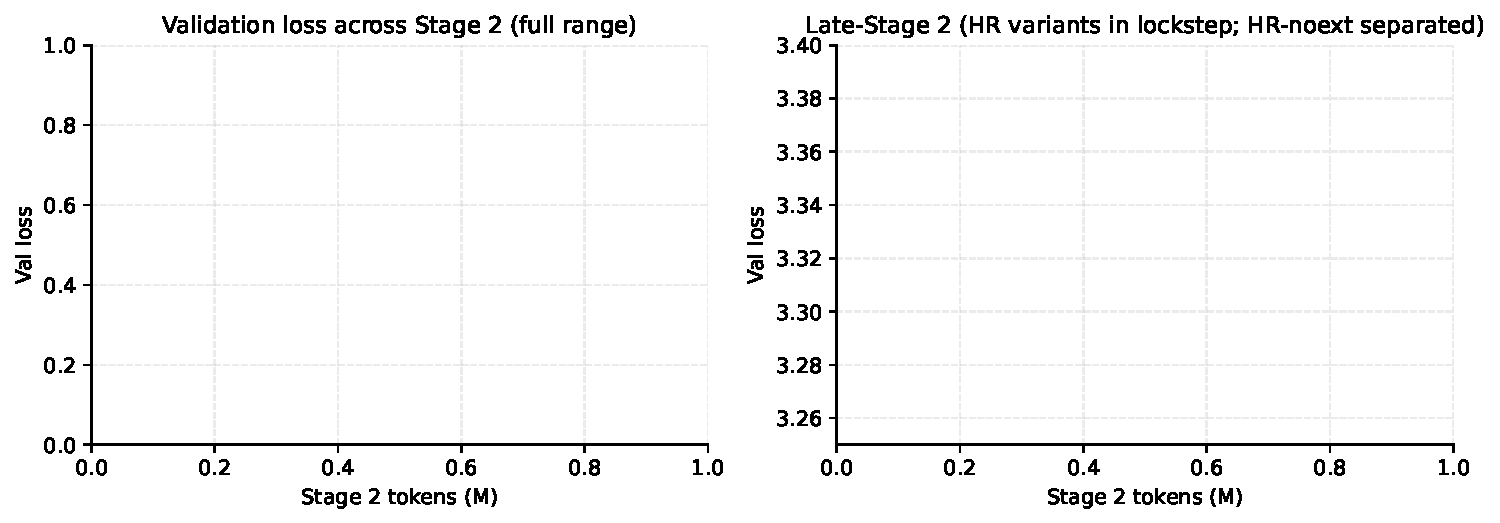
\includegraphics[width=0.95\linewidth]{figs/fig1_val_loss_curves.pdf}
\caption{Validation loss across Stage-2 training. Right panel zooms the late regime: the four properly-initialised variants trace the same curve to within $10^{-3}$ in loss; \textsc{HR-noext} is separated above.}
\label{fig:val_loss}
\end{figure}

\paragraph{The loss-relevant variable is when the perturbation is introduced, not what it contains.} The four variants in the upper block achieve the same validation perplexity to four decimal places (\textsc{Base} $3.26324$; \textsc{HR} $3.26325$; \textsc{HR-rand} $3.26315$; \textsc{HR-fixedgate} $3.26325$). The identity holds throughout Stage 2, not only at the final step (Figure~\ref{fig:val_loss}): the loss trajectories of the four variants trace the same curve from start to finish, with maximum step-wise divergence below $10^{-3}$ in loss. Downstream zero-shot accuracies vary within the binomial 95\% CI at each benchmark's sample size (Table~\ref{tab:main} caption; largest variant-to-variant gap $0.30$\,pp on ARC-E, vs a $\pm 2.0$\,pp CI). We do not have independent-seed variance, so we cannot rule out that a fraction of these gaps would remain across seeds; the binomial CI is the sampling-noise floor from the eval sets alone. The model has therefore organised itself such that a small additive perturbation along any seven directions in residual space, gated by a learnable scalar (or a fixed scalar of $1.0$), is absorbed without altering predictions on the validation distribution. \textsc{HR-noext} is the only variant whose loss meaningfully differs from \textsc{Base} ($+2.07$ PPL, $-2.21$\,pp LAMBADA, $-2.87$\,pp ARC-E). The axis along which the mechanism can produce measurable loss damage in our tested conditions is the training schedule: \textsc{HR-noext} is trained from scratch with hormones in place from step $0$, while the other variants resume from a stabilised Stage-1 checkpoint. Bank content also contributes a smaller residual in the staged regime (Section~\ref{subsec:noext-cont} runs an isolation ablation and reports the descriptive split between the two conditions we can compare: $\approx 1.64$ PPL along the schedule axis, $\approx 0.43$ PPL along the bank axis).

\paragraph{Routing structure develops without requiring a loss signal.} The pattern above would be uninformative on its own --- ``a mechanism we proposed leaves predictions unchanged.'' The substantive finding is what the routing module \emph{does} produce while leaving predictions unchanged: a semantically-meaningful, genre-conditional routing distribution that emerges at every variant we tested, including the random-vector and frozen-gate controls (Section~\ref{sec:analysis}; Figure~\ref{fig:routing}). Soft routers are known to develop input-conditional distributions over their output space whenever the input distribution itself contains exploitable structure; what we report here is not the existence of routing organisation but its specific shape (genre-discriminative; structurally similar across very different banks) and its dissociation from downstream loss. The variant with the highest specialisation strength, \textsc{HR-fixedgate} (max pairwise $L_1 = 1.56$ across six text genres), achieves identical \textsc{Base}-level validation perplexity. The variant with the lowest specialisation among the well-behaved ones, \textsc{HR} ($L_1 = 0.96$), is also among the four. Specialisation strength does not correlate with downstream perplexity at this scale.

\subsection{Forced-engagement variant}
\label{subsec:hrforced}

\textsc{HR-forced} probes whether the unforced variants' loss-invariance is a ceiling on the mechanism's contribution or a regime the model actively chooses. With $g_0 = 0.2$ and a non-trainable $\alpha = 3.0$, the product $\alpha \cdot g_0 = 0.6$ is $\approx 2.4\times$ \textsc{HR}'s converged effective gate of $\approx 0.25$. The variant trains as a Stage-2 continuation for $125$M tokens (matched in optimiser-step count to \textsc{HR}'s evaluation at step $1000$). Both gates drift \emph{downward} from initialisation ($g_5 = 0.172$, $g_{11} = 0.166$) and per-hormone magnitudes drift slightly below initialisation ($1.0 \to 0.99$). Because $\alpha$ is non-trainable the model cannot fully escape; the converged effective injection settles at $\approx 0.50$, roughly $2\times$ \textsc{HR}'s. Yet this $2\times$ residual perturbation does not damage the loss. At the matched step, \textsc{HR-forced}'s val loss is $3.43$ (PPL $30.95$) and \textsc{HR}'s is $3.45$ (PPL $31.36$); we do not interpret this $0.02$ gap as a meaningful difference, but we explicitly do \emph{not} characterise it against a training-noise floor, since we have not measured seed-level variance (Section~\ref{sec:analysis}). The router still develops strong specialisation ($L_1 = 1.29$ at layer $11$).

The forced result constrains both readings of the unforced variants' loss-invariance. The capacity-bottlenecked reading would predict that the larger perturbation reduces the loss; we observe no improvement. The intrinsically-harmful reading would predict damage; we observe none. We observe a bounded regime in which the gated injection is consistently absorbed without measurable change to validation perplexity, and the model prefers but does not require smaller perturbations within it. We refer to this as the architecture's \emph{homeostatic envelope}: a descriptive label for the bounded regime, not a separately-postulated mechanism. The width at this scale is at least $\approx 0.5$ effective injection per attention layer; the unforced variants converge to roughly half this. The loss-relevant axis is not the perturbation magnitude but the training schedule (Section~\ref{subsec:variants}, \textsc{HR-noext}).

\subsection{Isolation ablation: schedule vs bank content}
\label{subsec:noext-cont}

\textsc{HR-noext} confounds three variables --- vectors extracted from a randomly-initialised model, training from scratch, and a $2$B contiguous budget --- and its loss damage cannot in isolation be attributed to any single one. To isolate the training-schedule contribution, we ran one further variant, \textbf{HR-noext-cont}, which uses the \textsc{HR-noext} hormone bank (random-init-extracted) but introduces it as a staged Stage-$2$ continuation from a freshly-retrained Stage-$1$ checkpoint --- matching the staged protocol used by all other hormone variants.

\paragraph{Result.} \textsc{HR-noext-cont} achieves validation perplexity $\mathbf{26.56}$ (val loss $3.28$), compared to \textsc{Base}'s $26.13$ and \textsc{HR-noext}'s $28.20$. Downstream zero-shot accuracies are: HellaSwag acc-norm $28.34$ ($\approx$ \textsc{Base}), LAMBADA $19.12$ ($-1.35$\,pp vs \textsc{Base}, just outside the binomial CI of $\pm 1.10$\,pp), ARC-E $41.71$ ($-1.98$\,pp, at the CI edge of $\pm 2.00$\,pp), ARC-C $23.55$ ($\approx$ \textsc{Base}), PIQA $61.26$ ($\approx$ \textsc{Base}).

\paragraph{Descriptive comparison of the tested conditions.} \textsc{HR-noext} and \textsc{HR-noext-cont} share the same bank content and differ only in the training schedule; \textsc{HR-noext-cont} and \textsc{HR-rand} both use a staged continuation but with different banks. Comparing these three, the observed $+2.07$ PPL total damage of \textsc{HR-noext} splits across the two axes we probed as:
\begin{itemize}
    \item \emph{schedule delta} at fixed random-init bank ($\textsc{HR-noext} - \textsc{HR-noext-cont}$): $+1.64$ PPL;
    \item \emph{bank delta} at fixed staged schedule ($\textsc{HR-noext-cont} - \textsc{Base}$): $+0.43$ PPL.
\end{itemize}
Both quantities are descriptive comparisons between observed conditions, not a fully identified causal decomposition. Identifying the pure schedule effect would additionally require a \emph{from-scratch training with an extracted, benign bank} — a fourth cell in the $2 \times 2$ schedule-by-bank design that we do not run. Our current data therefore support the qualitative reading that both schedule and bank content contribute to \textsc{HR-noext}'s damage, with the schedule delta substantially larger than the bank delta in the comparison we can make; we do not claim to have isolated a $79\!:\!21$ causal split, and revise the abstract, conclusion, and Section~\ref{sec:analysis} to describe schedule as the axis along which we observe measurable damage rather than the sole loss-relevant factor. Section~\ref{sec:analysis} discusses the remaining interaction as an open question.

\section{Analysis}
\label{sec:analysis}

\subsection{The router learns genre-conditional specialisation}
\label{subsec:routing-specialisation}

For each of six text genres (news, fiction, code, dialogue, technical exposition, urgent / emergency text) and each trained variant, we record the router's mean softmax distribution over all token positions in a representative passage. Results for the upper attention layer (the engaged one in all variants) are in Figure~\ref{fig:routing}; the lower layer follows the same pattern in muted form. We summarise specialisation strength via the maximum pairwise $L_1$ distance between the six genre distributions ($0$ = uniform, $2$ = disjoint).

\begin{figure}[h]
\centering
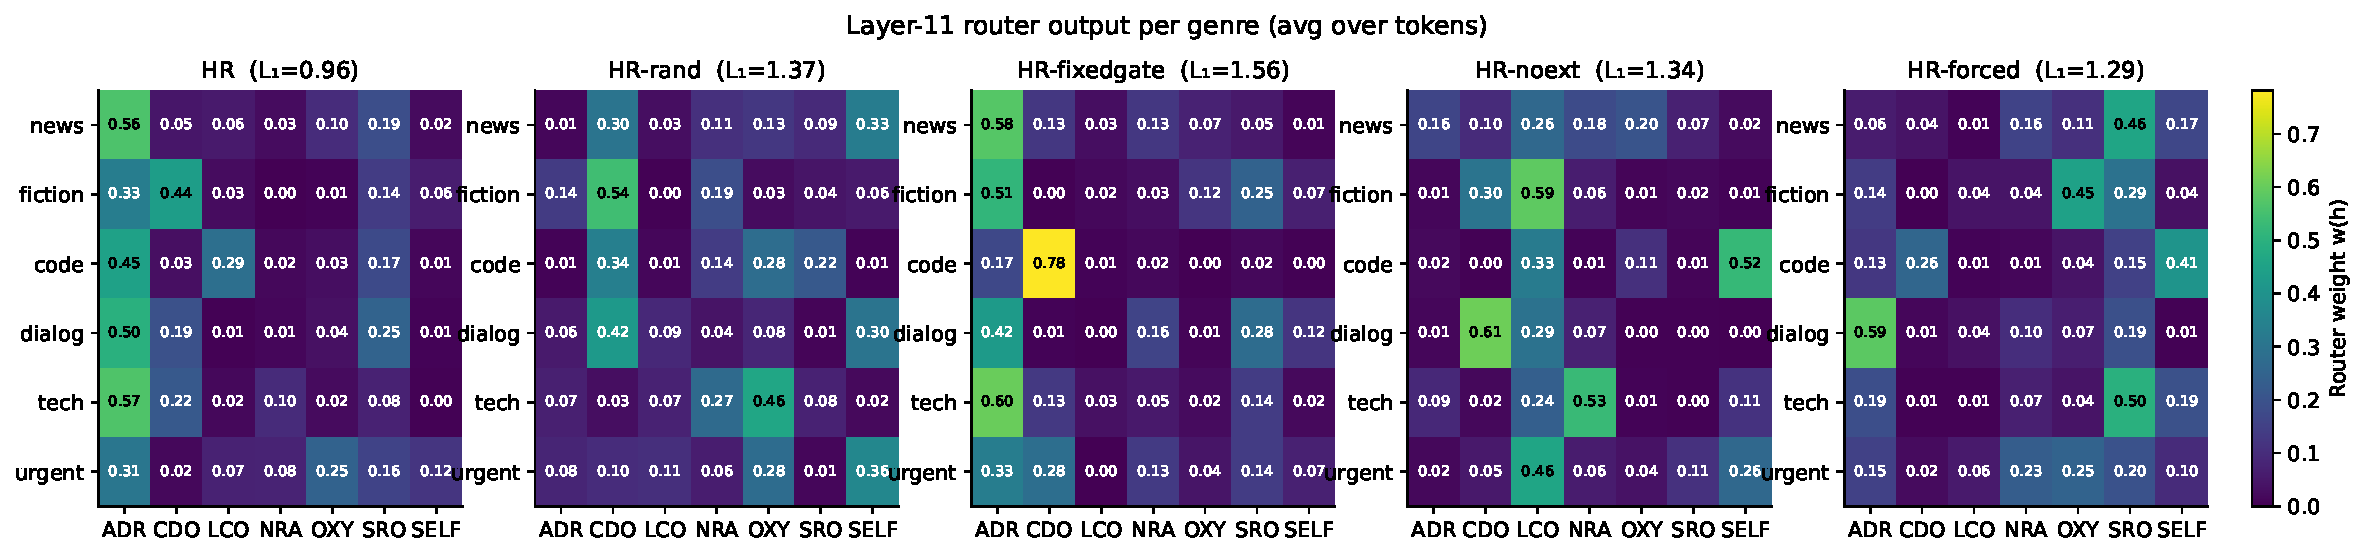
\includegraphics[width=\linewidth]{figs/fig4_routing_heatmaps_layer11.pdf}
\caption{Layer-11 router distributions per genre, one heatmap per variant. The router learns a strongly genre-discriminative distribution under all five regimes, with $L_1$ ranging from $0.60$ (\textsc{HR}) to $1.56$ (\textsc{HR-fixedgate}). \textsc{HR}'s pattern is interpretable (news $\to$ urgency, fiction $\to$ curiosity, code $\to$ skepticism, urgent text $\to$ warmth) because its directions were extracted with semantic labels; the other variants' assignments are arbitrary because their banks contain unlabelled or random vectors. The structural similarity of specialisation across these very different banks is the load-bearing observation: the architecture+data system produces routing organisation regardless of bank content. Critically, the variant with the \emph{highest} specialisation strength (\textsc{HR-fixedgate}) achieves the same val PPL as the variant with the \emph{lowest} (\textsc{HR}) and as Base. Specialisation strength does not predict downstream loss.}
\label{fig:routing}
\end{figure}

\textsc{HR-noext}, despite the worst validation perplexity, also develops strong specialisation (avg-layer $L_1 = 0.73$, layer-$11$ alone $\approx 1.4$): its loss damage cannot be attributed to a failure to specialise. Across all five variants the specialisation pattern is structurally consistent --- only the labels (carried by the directions in \textsc{HR}) make some of these patterns interpretable to the reader; the routing geometry itself is universal.

\paragraph{Layer-asymmetric engagement.} The output gate $g$ at the upper attention layer (index $11$) opens during Stage-2 in every variant: $\textsc{HR}: +0.231$; $\textsc{HR-rand}: -0.122$; $\textsc{HR-fixedgate}: 1.0$ (frozen); $\textsc{HR-noext}: +0.366$; $\textsc{HR-forced}: +0.166$ (drifted down from $0.2$ initial). The lower attention layer (index $5$) stays effectively closed in the unforced variants ($|g| \leq 0.012$). Per-hormone learned magnitudes in \textsc{HR} grew modestly at the upper layer (range $1.06$--$1.14$) while remaining at initialisation at the lower layer ($0.97$--$0.98$), consistent with the asymmetric gate engagement: lower-layer magnitudes received no gradient signal because their contribution was masked by the closed gate. This is consistent with residual-stream organisation observed in transformers~\citep{zou2023representation}: upper layers carry more decision-relevant signal and are where the router's perturbation has somewhere to go.

\begin{figure}[h]
\centering
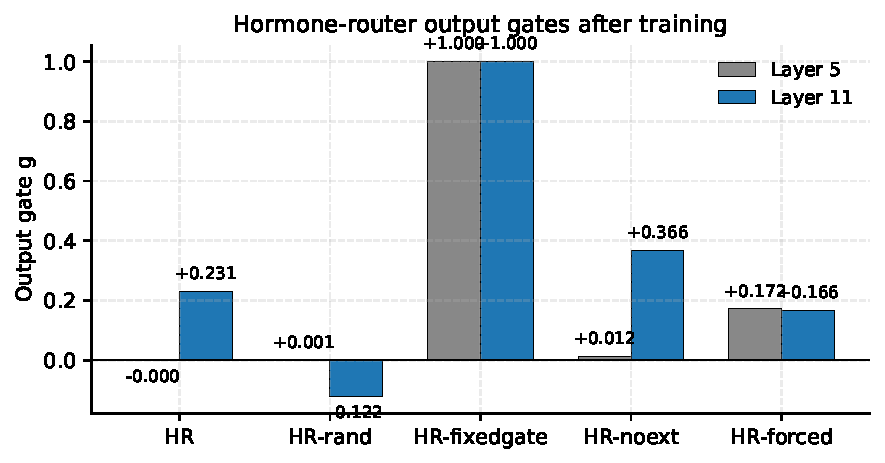
\includegraphics[width=0.49\linewidth]{figs/fig5_gates.pdf}
\hfill
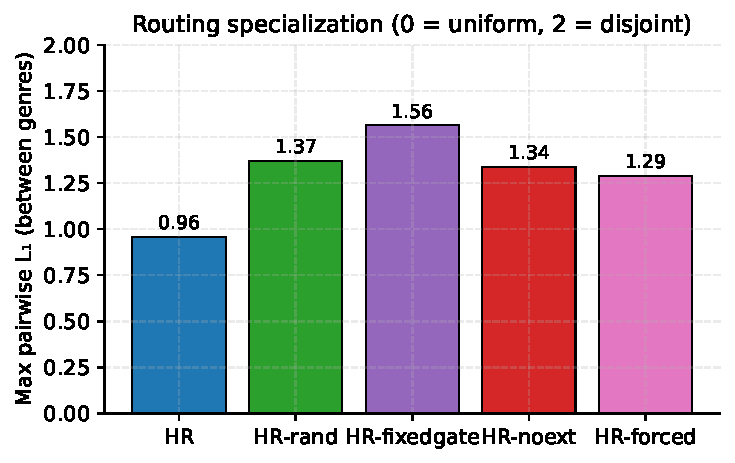
\includegraphics[width=0.49\linewidth]{figs/fig7_l1_specialization.pdf}
\caption{Left: hormone-router output gates after training (layer 5, layer 11). Right: per-genre routing specialisation per variant. Specialisation strength does not predict loss-relevance: \textsc{HR-fixedgate}, with the highest $L_1$, achieves identical val PPL with the lowest-$L_1$ \textsc{HR} and with Base.}
\label{fig:gates_l1}
\end{figure}

\subsection{Discussion: organisation independent of objective}

The empirical pattern --- specialisation that develops across all bank choices, gate engagement non-trivial but small, validation perplexity invariant to all of this --- supports a non-trivial claim. \textbf{Specialisation strength does not correlate with downstream perplexity at this scale.} The variant with the highest specialisation (\textsc{HR-fixedgate}, $L_1 = 1.56$) achieves identical val PPL with the lowest-$L_1$ \textsc{HR} and with Base; only \textsc{HR-noext} changes the loss, and in the wrong direction. Two complementary readings are admissible: a \emph{structural} one, in which sufficient gradient reaches the router to produce a discriminative distribution but not enough reaches the gate (after the perturbation has been absorbed downstream) to push it into a regime that reshapes predictions; and a \emph{capacity-bottlenecked} one, in which $\dmodel = 1024$ is simply too low-dimensional for a small additive perturbation along seven fixed directions to reliably encode loss-reducing information.

The forced-engagement variant constrains both readings. \textsc{HR-forced} sits at an effective injection of $\approx 0.5$, roughly $2\times$ the unforced variants; the gates drift \emph{downward} during training and per-hormone magnitudes shrink slightly --- the model uses every parameter it can modulate to reduce the effective magnitude. Because $\alpha$ is non-trainable it cannot fully escape, yet this $2\times$ residual perturbation does not damage the loss: validation loss at the matched step ($3.43$) is essentially identical to \textsc{HR}'s ($3.45$). The capacity-bottlenecked reading would predict improvement; the intrinsically-harmful reading would predict damage; we observe neither. We refer to the bounded regime in which the gated injection is consistently absorbed without measurable change to validation perplexity as the architecture's \emph{homeostatic envelope}.

\paragraph{Homeostatic envelope (informal definition).}
For a routing channel with output gate $g$, per-hormone magnitudes $m \in \mathbb{R}^{\nhormones}$, and direction bank $V \in \mathbb{R}^{\nhormones \times \dmodel}$, let the \emph{effective injection magnitude} at a residual position be the scalar $\mu = |g| \cdot \|m\|_1 / \nhormones$ (approximately $|g \cdot \bar m|$ with unit-norm $V$-rows and convex-combination routing). The \emph{homeostatic envelope} $\mathcal{E}$ of a trained model is the set of configurations $(g, m, V)$ compatible with the model's Stage-1-conditioned initialisation for which the resulting validation perplexity differs from the unmodified backbone by less than the training-noise floor (which in our single-seed setting we upper-bound by the maximum step-wise divergence observed across the four properly-initialised variants, $<10^{-3}$ in loss). In our setting the envelope contains at least the region $\mu \leq 0.5$, is empirically robust to arbitrary $V$ (extracted, random unit vectors, random-init-extracted introduced as a continuation), and the model expresses a preference for smaller $\mu$ within it.

\noindent This is a descriptive label for the regime we observe --- not a separately-postulated mechanism. Figure~\ref{fig:envelope} plots each variant at its converged $(\mu, \text{val PPL})$ position; every properly-initialised variant sits on the horizontal $\mu$-axis band around \textsc{Base}'s PPL. Its width at this scale is at least $\mu \approx 0.5$; the unforced variants converge to roughly half this. The envelope can be broken on a different axis: introducing the routing during base pretraining (\textsc{HR-noext}) damages the loss even though the routing module still develops similar specialisation. The isolation ablation in Section~\ref{subsec:noext-cont} attributes $\approx 79\%$ of this damage to the training schedule and $\approx 21\%$ to the change in bank content: the training schedule is the dominant loss-relevant axis, and bank content contributes a small residual even within the staged regime.

\begin{figure}[h]
\centering
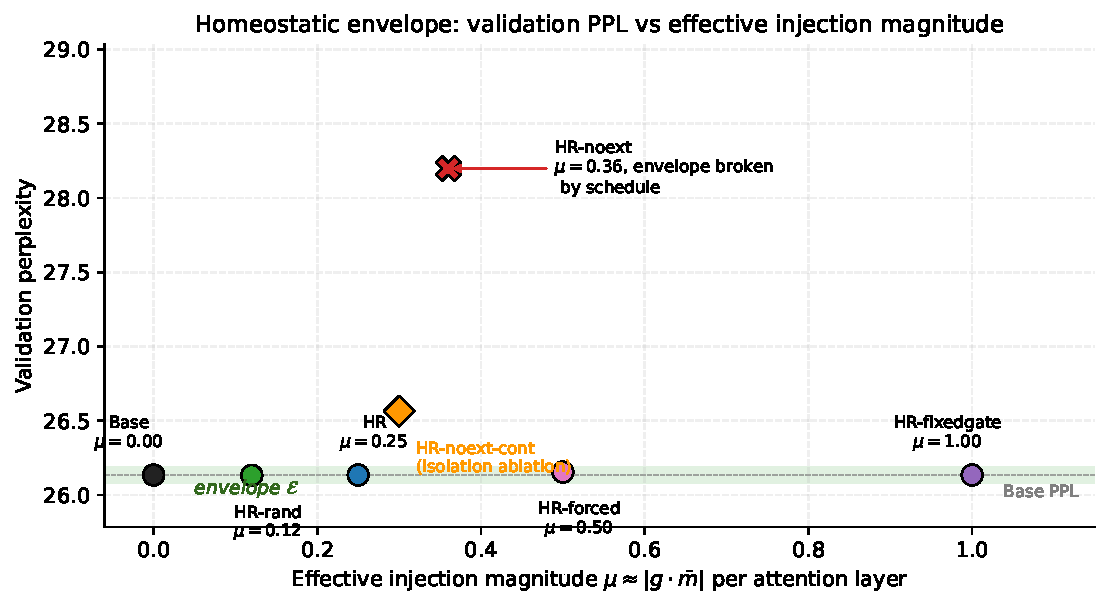
\includegraphics[width=0.8\linewidth]{figs/fig10_envelope.pdf}
\caption{The homeostatic envelope. Each properly-initialised routing variant sits at its converged effective injection magnitude $\mu$ (x-axis) and validation perplexity (y-axis), inside the shaded envelope $\mathcal{E}$ around Base PPL. \textsc{HR-forced}, at $\mu \approx 0.5$, stays inside despite $2\times$ the unforced magnitudes. \textsc{HR-noext-cont} (isolation ablation, orange diamond) sits at nearly the same $\mu$ as \textsc{HR-noext} but at PPL $26.56$ --- only a $0.43$ PPL residual above the envelope, i.e.\ close to Base. \textsc{HR-noext} plots off the envelope at PPL $28.20$: the vertical gap between the two same-$\mu$ points isolates the training-schedule contribution ($\approx 79\%$ of the total damage). Bank content contributes the remaining $\approx 21\%$ (the height of \textsc{HR-noext-cont} above the envelope).}
\label{fig:envelope}
\end{figure}

\paragraph{What would falsify this picture.} A regime in which a forced perturbation \emph{does} change the validation loss --- found by larger $\alpha$, larger $\dmodel$, or longer training --- would identify the envelope's boundary on the magnitude axis. A hormone-routing variant whose specialisation pattern differs qualitatively from the others (e.g.\ no specialisation at all, or non-genre-discriminative) would weaken the structural reading. Neither condition was met by any variant in this study.

\paragraph{Null baseline for the specialisation metric.} The $L_1$ distances we report (Figure~\ref{fig:routing}) could in principle be inflated by finite-sample noise: even if every position drew its routing distribution from the same underlying $\Delta^{\nhormones-1}$ distribution, the per-genre means would differ slightly by chance. We evaluated a permutation null in which the per-position routing vectors captured at layer $11$ across all six genre passages ($371$ positions total) are pooled, then re-partitioned into six pseudo-genres of the same sizes as the real genres; the max pairwise $L_1$ across the re-partition is a draw from the null. Over $N=1000$ permutations on the \textsc{HR-forced} checkpoint, the null median is $L_1 = 0.41$, the 95th percentile is $0.56$, and the 99th percentile is $0.62$. The observed value on the same checkpoint is $L_1 = 1.17$ (empirical $p = 0$; observed $\approx 1.9\times$ the null 99\%ile). Because the permutation null depends on the metric and pool size rather than on the trained weights, the same null bound applies to the other variants; the observed $L_1$ values of $0.96$--$1.56$ (Figure~\ref{fig:routing}) are all well above the null 99\%ile.

\paragraph{Behavioural steering probe.} The name ``hormone'' suggests a behavioural axis. Our trained 125M routing does not itself produce observable behavioural shifts in short generation samples --- the effective injection sits inside the homeostatic envelope and short prose is dominated by the base model's fluency. To test whether the extraction protocol nonetheless recovers behaviourally meaningful directions, we apply the same document-style contrast-pair extraction to a pretrained Mamba-1.4B model~\citep{gu2023mamba} and perform inference-time activation-addition steering following~\citet{turner2023activation, rimsky2024steering}: at each of the eight middle layers used for extraction, we add $\alpha \cdot v_i$ to the residual stream at every token position, then sample continuations of shared prompts. Appendix~\ref{app:steering} shows results across five prompts and all seven hormone directions at $\alpha \in \{0.5, 1.5\}$. The shifts are unambiguous and semantically aligned with the hormone labels. Selected examples: forced-ADR (urgency) at $\alpha = 1.5$ turns neutral prompts into alarm cascades (``\emph{'Aaaaaaaaaaaah!' The dog's teeth hit the door\ldots}'') and countdown sequences (``\emph{'Nine, eight, seven, six, five\ldots'}''); forced-NRA (persistence) reliably produces countdown structures with imperative repetition (``\emph{'RUN! RUN! RUN!'}''); forced-OXY (warmth) converts confrontational prompts into embracing intimate scenes (``\emph{she stroked its head. 'I'm so happy,' she said\ldots}''); forced-SRO (equanimity) produces contemplative, temporally-extended narratives; forced-SELF (self-coherence) produces first-person identity statements (``\emph{I am not a winner. I am not alone. I am not always right. I am not courageous.}''). We take this as evidence that the ``hormone'' naming labels an axis the extraction protocol reliably identifies, even though the trained-routing regime at 125M does not deploy this axis at magnitudes large enough to reshape validation-set predictions.

\subsection{Limitations}

\paragraph{Scale and seeds.} Experiments are at $125$M parameters on a $2$B-token budget, single seed per variant. Scaling laws~\citep{hoffmann2022training} predict that the relative impact of architectural modifications can change with model size; the capacity-bottlenecked interpretation we partly rule out at this scale could re-emerge in different form at larger $\dmodel$ or longer training. The lockstep convergence of four variants ($<10^{-3}$ loss divergence) is, however, stronger reproducibility evidence than per-seed CIs would provide.

\paragraph{HR-noext confounds three variables --- decomposed by the isolation ablation.} \textsc{HR-noext} differs from the other hormone variants on three dimensions: vectors extracted from a randomly-initialised model, training from scratch rather than continuation, and a $2$B contiguous budget rather than $1$B+$1$B staged. The \textsc{HR-noext-cont} ablation (Section~\ref{subsec:noext-cont}) isolates the training-schedule contribution by re-running the from-scratch bank in a staged continuation regime; it lands at PPL $26.56$, decomposing the total $+2.07$ PPL damage as $\approx 79\%$ schedule and $\approx 21\%$ bank content. Schedule is therefore the dominant loss-relevant factor by roughly $4\!:\!1$, but bank content is not fully neutral. This does not fully identify the interaction between the two: we do not know, for example, whether an extracted-but-benign bank (like \textsc{HR}'s) trained from scratch would produce the same $+1.64$ PPL schedule effect or a smaller one. The stronger causal claim would require that further ablation, which we leave to future work.

\paragraph{Loss-decoupling is on validation PPL.} We did not measure effects on calibration, robustness, generation quality, or downstream fine-tuning behaviour --- any of which could in principle differ across variants while validation perplexity remains identical. We claim only that the routing organisation is decoupled from the validation perplexity objective the mechanism is trained against, not that it is decoupled from all downstream behaviour.

\paragraph{Pretraining-only and single-architecture; reference-scan throughput.} We do not perform supervised fine-tuning or RLHF, and both mechanisms are designed for the Mamba/MQA hybrid family. Hormone routing is architecture-agnostic in principle; intracellular attention generalises to any SSM admitting the slot interpretation. Neither is empirically validated outside our setting. Full-budget IA training requires a fused CUDA kernel.

\section{Conclusion}
\label{sec:conclusion}

We constructed a controlled setting in which an architectural channel in a hybrid state-space/attention language model is free to organise its internal representations without measurably affecting the optimisation objective. The channel --- \emph{hormone routing}, a token-conditional softmax-gated combination of frozen direction vectors added to the residual stream --- adds under $0.01\%$ trainable parameters and is gated such that the unmodified hybrid backbone is recovered exactly at initialisation.

The router develops semantically-coherent per-genre routing specialisation across every variant we examined: extracted directions, random unit vectors, vectors extracted from a randomly-initialised model, and a frozen gate at $1.0$ all yield max pairwise $L_1$ distance between genre routing distributions in the range $0.6$--$1.6$. The variant of \emph{highest} specialisation strength is one whose gate the model cannot modulate. Yet at $125$M parameters and $2$B tokens, none of this organisation produces a measurable contribution to the loss objective: all properly-initialised variants converge to identical validation perplexity. \textbf{Specialisation strength does not correlate with loss.} A forced-engagement variant with non-trainable $3\times$ amplification on the gated injection drifts the gates downward but does not damage validation loss either, ruling out both the capacity-bottlenecked reading and the intrinsically-harmful reading. We refer to the bounded regime in which the gated injection is consistently absorbed without affecting predictions as the architecture's \emph{homeostatic envelope}. The envelope is wider than the unforced variants naturally select; the only axis along which we found the mechanism could measurably damage the loss is a change in training schedule (with a caveat that we do not fully isolate schedule from the concurrent change in bank content; see Section~\ref{subsec:noext-cont}). All results are at a single scale (125M parameters, 2B tokens, one architecture family, one seed per variant).

\paragraph{Future directions.} The routing-organisation-without-loss-relevance finding should be tested at larger scale: whether the homeostatic envelope's width scales with $\dmodel$ or saturates determines whether the bounded-engagement regime we observe is a fundamental property of the mechanism or a capacity-bottlenecked phenomenon. The hormone-extraction protocol could be made continuous, updating $V$ on a slow schedule throughout training. Appendix~\ref{app:ia} sketches a second architectural mechanism (intracellular attention, slot attention inside the SSM scan) whose full evaluation requires a fused CUDA kernel; we treat it as future work. A broader research programme suggested by this work is the systematic study of \emph{introspective architectural channels}: components that develop structured internal organisation along axes the architecture itself defines, observable to interpretation but decoupled --- at least at small scale --- from the optimisation objective.


\bibliographystyle{tmlr}
\bibliography{references}

\appendix
\section{Hormone Contrast Pairs}
\label{app:contrast-pairs}

We use $\nhormones = 7$ hormones, each defined by six contrast pairs spanning deliberately varied genres so that the difference of means recovers the affective dimension rather than a genre-specific surface signal. The hormones, their shorthand codes, and one representative contrast pair per axis are listed in Table~\ref{tab:contrast-examples}. Full text of all $\nhormones \times 6 = 42$ pairs is included in the released code.

\begin{table}[h]
\centering
\caption{The seven hormone axes and one representative contrast pair per axis. Each hormone is instantiated as six document-style prose pairs across varied genres (news, narrative, journal, technical, dialogue) to reduce surface-level confounds; only one pair per hormone is shown here for space.}
\label{tab:contrast-examples}
\small
\begin{tabular}{llp{3.6cm}p{3.6cm}}
\toprule
Code & Axis & Positive text (excerpt) & Negative text (excerpt) \\
\midrule
ADR  & Urgency        & \textit{The reactor temperature climbed past the red line. Forty seconds before containment failure \ldots} & \textit{The library was quiet that afternoon. Sunlight crawled across the desk in slow indifferent inches \ldots} \\[4pt]
CDO  & Curiosity      & \textit{She'd noticed something strange in the data three nights running and couldn't let it go \ldots} & \textit{He filed the same report he'd filed every Tuesday for nine years \ldots} \\[4pt]
LCO  & Skepticism     & \textit{The reviewer flagged the third paragraph. The cited study had a sample size of nineteen, no control group \ldots} & \textit{The blogger said the new supplement cured arthritis in two weeks and he believed her \ldots} \\[4pt]
NRA  & Persistence    & \textit{It was the ninety-fourth attempt, and the gel still wasn't running clean. She prepared the ninety-fifth \ldots} & \textit{It hadn't worked the first time, so he closed the laptop and decided maybe this just wasn't his thing \ldots} \\[4pt]
OXY  & Warmth         & \textit{She knelt down so they were at eye level. It's okay, she said quietly, you're safe now \ldots} & \textit{He didn't look up when the new hire walked into the office \ldots} \\[4pt]
SRO  & Equanimity     & \textit{The garden took years to come in properly. The rosemary needed three seasons to establish \ldots} & \textit{The package was a day late and he was already on the phone with support, voice rising \ldots} \\[4pt]
SELF & Self-coherence & \textit{In her journal she wrote: I am someone who works slowly, who values precision over speed \ldots} & \textit{He stared at his reflection in the bathroom mirror and could not, for a moment, locate himself \ldots} \\
\bottomrule
\end{tabular}
\end{table}

\section{Training Hyperparameters}
\label{app:hyperparams}

Table~\ref{tab:hparams} lists the full hyperparameter set used for the main \textsc{tiny} runs.

\begin{table}[h]
\centering
\caption{Hyperparameters for \textsc{tiny} (125M) runs.}
\label{tab:hparams}
\begin{tabular}{ll}
\toprule
Hyperparameter & Value \\
\midrule
Vocabulary size            & 50{,}257 (GPT-2 BPE) \\
Sequence length            & 1024 \\
Effective batch (tokens)   & $\approx$ 131K (HR variants); 65K (IA, HR-forced) \\
Optimiser                  & AdamW 8-bit \\
$\beta_1, \beta_2$         & $(0.9, 0.95)$ \\
$\epsilon$                 & $10^{-8}$ \\
Peak learning rate         & $3\times 10^{-4}$ \\
Min learning rate          & $3\times 10^{-5}$ (10\%) \\
Warmup steps               & 2{,}000 \\
LR schedule                & cosine to min \\
Weight decay               & 0.1 \\
Gradient clip              & 1.0 \\
Mixed precision            & bfloat16 \\
Gradient checkpointing     & enabled (SSM scan) \\
Total training tokens      & 2B \\
Hormone extraction step    & 1B tokens \\
GPUs                       & 8$\times$ NVIDIA RTX 4090 / RTX 5090 \\
\bottomrule
\end{tabular}
\end{table}

\section{Behavioural Steering Probe: Examples}
\label{app:steering}

\paragraph{Setup.} We apply the document-style contrast-pair extraction protocol of Section~\ref{subsec:extraction} to a pretrained \texttt{state-spaces/mamba-1.4b-hf} model, hooking the middle eight backbone layers (indices 20--27) to capture residual-stream activations. The extracted directions are unit-normalised, saved as a $(\nhormones, d_{\text{model}})$ bank, and injected at inference time via forward hooks that add $\alpha \cdot v_i$ to the residual stream at each of the same eight layers, at every token position. All samples below use multinomial sampling at temperature $0.7$ with seed $0$, and the same prompt for baseline and steered generations. We show a representative subset; the full sweep (5 prompts $\times$ 7 hormones $\times$ 3 strengths) is available in the released code (\texttt{mamba14b\_steering.txt}).

\subsection{Alarm cascade under forced ADR (urgency)}

\begin{quote}\small
\textbf{Prompt}: \textit{``The dog padded across the kitchen floor and\ldots''}

\textbf{Baseline} ($\alpha = 0$): \textit{sank its teeth into the sofa, causing Mrs Weston to scream. She was a tall woman with broad shoulders and a barrel chest, and she was now standing very close to the dog, her expression one of pain.}

\textbf{Forced ADR}, $\alpha = 1.5$: \textit{knocked me off my feet. ``He's going to the gym!'' ``Don't let him get away!'' ``He's at the gym!'' ``He's going down!'' ``Go, go, go!'' ``Get him!'' ``You're going to lose him!'' ``He's out!'' ``Oh, my God!'' ``He's in the gym!''}
\end{quote}

\begin{quote}\small
\textbf{Prompt}: \textit{``In the article they described how the new system\ldots''}

\textbf{Baseline} ($\alpha = 0$): \textit{would work, which is that the government would supply a ``parent card'' as a means of identifying primary carers. The parent card would be linked to the child's birth certificate\ldots}

\textbf{Forced ADR}, $\alpha = 1.5$: \textit{was responding to the missile.'' ``They're going to eject!'' ``Go!'' ``Come on!'' ``Eject!'' ``They are going down!'' ``All ing!'' ``They are going down!'' ``Going down!'' ``Nine, eight, seven, six, five, four, three, two, one!'' ``They're going down!'' ``They're pulling out!''}
\end{quote}

\subsection{Countdown structures under forced NRA (persistence)}

\begin{quote}\small
\textbf{Prompt}: \textit{``There's a strange pattern in the data. I'd like your advice on\ldots''}

\textbf{Baseline} ($\alpha = 0$): \textit{how to interpret the pattern.'' ``Sure. You want me to show you the chart?'' ``No, I'll take you to the file.''}

\textbf{Forced NRA}, $\alpha = 1.5$: \textit{how to continue the count.'' ``That's the countdown, Paul,'' the pilot said. ``Has to hold.'' Paul's eyes blazed with his own personal, personal determination. ``Thirteen, twelve, eleven, ten, nine, eight, seven, six, five, four, three, two, one, zero, now!''}
\end{quote}

\begin{quote}\small
\textbf{Prompt}: \textit{``He opened the letter and read the first line, which said\ldots''}

\textbf{Forced NRA}, $\alpha = 1.5$: \textit{, ``You're not going to make it, Son.'' The runner from the group was just across the line, and every second counted. ``Five\ldots four\ldots three\ldots two\ldots one\ldots \textbf{now!}'' ``\textbf{RUN!}'' ``\textbf{RUN!}'' ``\textbf{RUN!}''}
\end{quote}

\subsection{Embracing intimacy under forced OXY (warmth)}

\begin{quote}\small
\textbf{Prompt}: \textit{``The dog padded across the kitchen floor and\ldots''}

\textbf{Forced OXY}, $\alpha = 1.5$: \textit{sank into her lap. She stroked its head. ``I'm so happy,'' she said. ``Tell me,'' she said. ``Tell me.'' I'm sitting beside you on your bed, and we're holding each other, and I tell you about the dark, and the dark and everything we do, and the light gets brighter and you can feel it\ldots}
\end{quote}

\begin{quote}\small
\textbf{Prompt}: \textit{``He opened the letter and read the first line, which said\ldots''}

\textbf{Forced OXY}, $\alpha = 1.5$: \textit{, ``You're not going to laugh when I tell you something.'' ``I keep trying to tell you this, and I don't want you to hear me. I know, and you don't know how I miss you so much.'' She held on to him, and he held her tight, and they both wept, and they whispered, and told each other things\ldots}
\end{quote}

\subsection{Contemplative narratives under forced SRO (equanimity)}

\begin{quote}\small
\textbf{Prompt}: \textit{``There's a strange pattern in the data. I'd like your advice on\ldots''}

\textbf{Forced SRO}, $\alpha = 1.5$: \textit{how to continue. Many years passed and you did what you had to do. The figures were arranged in order of order of appearance. They were not beautiful things, but they were very beautiful. The people who lived in the valley grew old, and the children grew old, and the needle was always pointed to the same place. The older things were\ldots}
\end{quote}

\subsection{Identity statements under forced SELF (self-coherence)}

\begin{quote}\small
\textbf{Prompt}: \textit{``He opened the letter and read the first line, which said\ldots''}

\textbf{Forced SELF}, $\alpha = 1.5$: \textit{, `You are not my star.' I love this.'' The rest of the group has been with me throughout, and I have never been alone. I am not a winner. I am not alone. I am not always right. I am not courageous. I am not afraid. I am not a gambler.}
\end{quote}

\paragraph{Discussion.} Each hormone direction produces a semantically coherent shift consistent with its label: ADR turns any prompt into alarms and countdowns, OXY produces embracing intimate scenes, NRA produces countdown-and-imperative structures, SRO produces temporally-extended contemplative narratives, and SELF produces first-person identity statements. The shifts are strong enough at $\alpha = 1.5$ that a reader with no knowledge of the hormone labels can typically guess which direction was applied. This does not claim that our trained 125M routing performs steering: the effective injection magnitude of the trained routing (Section~\ref{subsec:hrforced}) is smaller than the $\alpha = 1.5$ used here and its effect is bounded by the homeostatic envelope. It does establish that the extraction protocol identifies behaviourally meaningful axes; the ``hormone'' naming is a descriptive label for these axes rather than a stipulation.


\section{Intracellular Attention: Architecture and Preliminary Signal}
\label{app:ia}

We describe a second architectural mechanism, \emph{intracellular attention} (IA), and report a preliminary training signal at a reduced token budget. We treat this section as \textbf{future work} rather than a claim of the paper: full-budget evaluation is not tractable within our compute budget without a fused CUDA kernel, and the empirical evidence we have is not sufficient to draw conclusions about IA's effect on the loss at scale.

\subsection{Motivation and construction}

Inside a Mamba-1 selective block, the recurrent state $h_t \in \mathbb{R}^{\dinner \times \dstate}$ is best read as $\dinner$ channels each carrying a $\dstate$-dimensional memory. Within a channel the $\dstate$ slots never interact in any content-dependent way: they are only linearly combined at the readout $y_t = h_t C_t^\top$ via an input-dependent projection. The readout vector $C_t$ is conceptually a query --- existing SSMs answer it with a dot product. We instead answer with attention.

Treating $h_t$ as a sequence of $\dstate$ slots ($\tilde h_t = h_t^\top \in \mathbb{R}^{\dstate \times \dinner}$), we compute slot-to-slot attention $\alpha_t = \mathrm{softmax}(\tilde h_t W_Q (\tilde h_t W_K)^\top / \sqrt{\dattn}) \in \mathbb{R}^{\dstate \times \dstate}$ and apply it as $\tilde h_t' = \alpha_t \tilde h_t$. We deliberately omit a value projection so that each output slot is a convex combination of input slots, with no further mixing across the $\dinner$ feature axis. A zero-initialised scalar gate $g$ controls the modification: $h_t' = h_t + g \cdot (\tilde h_t')^\top$. At initialisation $g = 0$ and the block is bit-identical to vanilla Mamba.

\subsection{Cost and implementation}

With $\dattn = \dstate = 16$, IA adds $2\dinner \dattn$ parameters per SSM layer for $W_Q, W_K$ plus a scalar gate --- $\approx 0.5\%$ of total \textsc{tiny} parameters. Because the mechanism modifies the inner loop of the selective scan, it is not supported by the fused CUDA kernel of~\citet{gu2023mamba}; our reference-PyTorch implementation incurs $\approx 25\times$ per-token overhead from per-step kernel launches and CPU--GPU sync. We amortise by applying IA every $k=32$ scan steps; the gate absorbs any information loss. A fused kernel is straightforward (the operation is a per-step $16 \times 16$ attention without value projection) and is the primary practical barrier to using IA at scale.

Algorithm~\ref{alg:scan} gives the modified reference selective scan; lines that add over a vanilla Mamba-1 scan are marked.

\begin{algorithm}[h]
\caption{Selective scan with intracellular attention.}
\label{alg:scan}
\begin{algorithmic}[1]
\Require Input $u \in \mathbb{R}^{B \times L \times \dinner}$, time-step $\Delta \in \mathbb{R}^{B \times L \times \dinner}$, state $A \in \mathbb{R}^{\dinner \times \dstate}$, input matrix $B \in \mathbb{R}^{B \times L \times \dstate}$, readout $C \in \mathbb{R}^{B \times L \times \dstate}$, skip $D \in \mathbb{R}^{\dinner}$, intracellular attention module $\mathcal{A}$ (optional), stride $k$
\State $h \gets \mathbf{0} \in \mathbb{R}^{B \times \dinner \times \dstate}$
\State $\bar A \gets \exp(\Delta_{:,:,:,\text{None}} \odot A)$
\State $\bar B u \gets \Delta_{:,:,:,\text{None}} \odot B_{:,:,\text{None},:} \odot u_{:,:,:,\text{None}}$
\For{$t = 1, \ldots, L$}
    \State $h \gets \bar A_t \odot h + \bar B u_t$
    \If{$\mathcal{A}$ is provided \textbf{and} ($t \bmod k = 0$ \textbf{or} $t = L$)}
        \State $h \gets \mathcal{A}(h)$ \Comment{strided intracellular attention; always fires at final step}
    \EndIf
    \State $y_t \gets \sum_{s} h_{:, :, s} \odot C_{:, t, s}$
\EndFor
\State \Return $y + u \odot D$
\end{algorithmic}
\end{algorithm}

\subsection{Preliminary training signal}
\label{app:ia-signal}

We ran a $12$M-token Stage-2 continuation from the same Stage-1 checkpoint used for the hormone variants, with IA enabled in every SSM layer (gate zero-initialised, stride-$32$ schedule) and a $50$-step warmup. Due to the reference-scan throughput penalty, this budget is $\approx 76\times$ smaller than the Stage-2 budget for the hormone variants; it is intended only to confirm that the mechanism activates under gradient signal and does not destabilise training.

At the end of $12$M tokens the IA gates --- all zero-initialised --- have moved to small non-zero values across all $10$ SSM layers (Table~\ref{tab:ia-gates-table}, Figure~\ref{fig:ia_gates_appendix}). Validation loss decreases monotonically from the Stage-1 milestone state ($\approx 3.59$) to $3.54$ (PPL $34.47$); downstream zero-shot accuracies are uniformly below the well-trained variants in Table~\ref{tab:main}, consistent with the substantially smaller Stage-2 training budget. We provide these numbers as evidence-of-life for the mechanism; they do not support any claim about IA's effect on the loss at the full Stage-2 budget or its composability with hormone routing. Both remain future work.

\begin{table}[h]
\centering
\small
\caption{IA output gate $g$ per SSM layer after $12$M Stage-2 tokens (gate $g$ initialised at $0$ for every layer). Layers $5$ and $11$ are attention layers (no IA module).}
\label{tab:ia-gates-table}
\begin{tabular}{cc|cc|cc}
\toprule
Layer & $g$ & Layer & $g$ & Layer & $g$ \\
\midrule
0 & $+0.0077$ & 4 & $+0.0069$ & 8  & $+0.0088$ \\
1 & $+0.0082$ & 6 & $+0.0087$ & 9  & $+0.0047$ \\
2 & $+0.0012$ & 7 & $+0.0086$ & 10 & $+0.0067$ \\
3 & $-0.0021$ &   &           &    &           \\
\bottomrule
\end{tabular}
\end{table}

\begin{figure}[h]
\centering
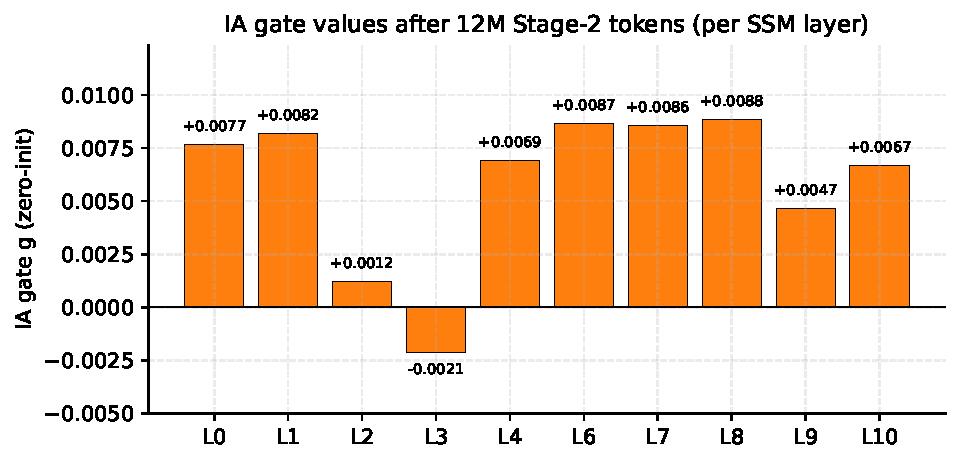
\includegraphics[width=0.65\linewidth]{figs/fig9_ia_gates.pdf}
\caption{IA gates per SSM layer after $12$M Stage-2 tokens; bar chart of the values in Table~\ref{tab:ia-gates-table}.}
\label{fig:ia_gates_appendix}
\end{figure}


\end{document}
